\documentclass{article}
\usepackage{graphicx} 
\usepackage{pgf-pie}
\usepackage[colorlinks=true, urlcolor=blue]{hyperref}

\title{Course logistics}
\date{}

\begin{document}

\maketitle


\section{DSA (CS213 and CS293)}

    \subsection{Course Website}

        \subsubsection{CS213 (Theory)}
        Lecture Slides : \\\url{https://robin.bodhi.cse.iitb.ac.in/courseware/course/195/content/multimedia/coursecontent/}

        \subsubsection{CS293 (Lab)}
        Labs : \\
        \url{https://robin.bodhi.cse.iitb.ac.in/courseware/course/195/content/labs}
        \\\\
        Lab seat mapping : \\\url{https://bit.ly/A26-DSA-Mapping}
        \\\\
        Crib form : \\\url{https://forms.gle/nTp4kmtFvKHQEVCW6 }
    \subsection{Quizzes}

        \subsubsection{CS213 (Theory)}
        Theory Quiz 1 : Thusday, 27th August 2026 (Lecture Slot)\\
        Midsem : Saturday, 12th September 2026 (5-7 PM)
        \subsubsection{CS293}
        Lab Quiz 1 : Tuesday, 25th August 2026 (Lab Slot)\\
        Midsem : Tuesday, 8th September 2026 (Lab Slot)
    \subsection{Grade Distribution}

        \subsubsection{CS213 (Theory)}
        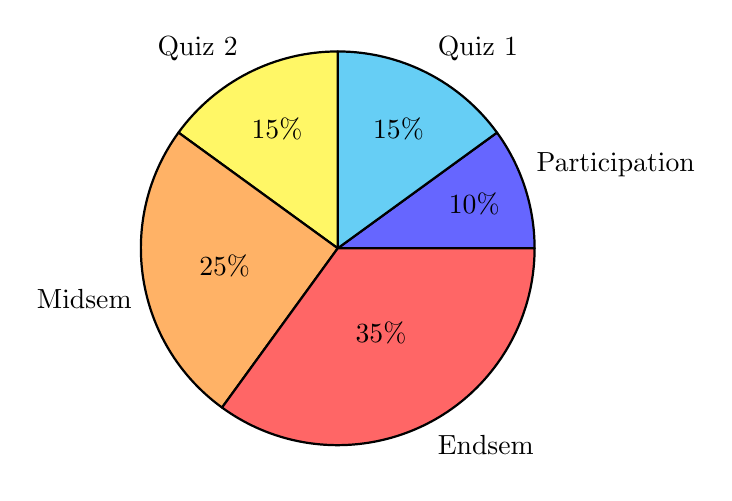
\begin{tikzpicture}
        \pie[radius=2.5]{10/Participation, 15/Quiz 1, 15/Quiz 2, 25/Midsem, 35/Endsem}
        \end{tikzpicture}

        \subsubsection{CS293 (Lab)}
        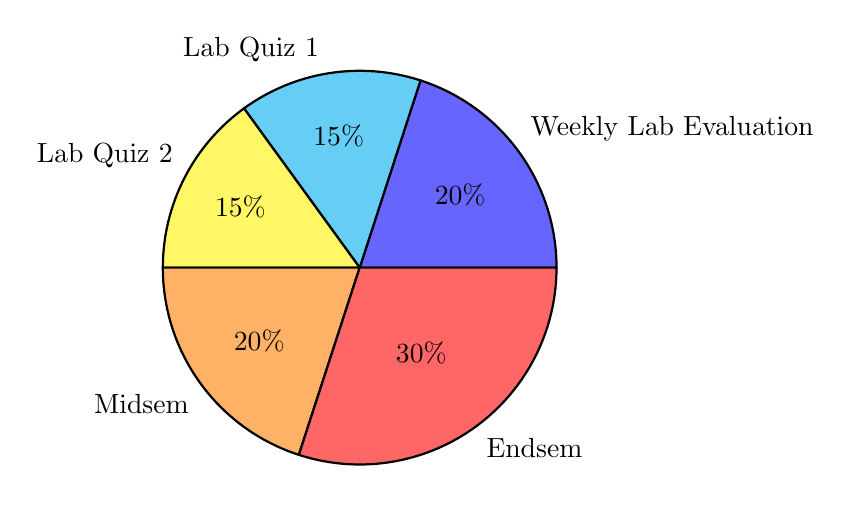
\begin{tikzpicture}
        \pie[radius=2.5]{20/Weekly Lab Evaluation, 15/Lab Quiz 1, 15/Lab Quiz 2, 20/Midsem, 30/Endsem}
        \end{tikzpicture}

    

\pagebreak


\section{DLDCA (CS230 and CS231)}

    \subsection{Course Websites}

        \subsubsection{CS230 (Theory)}
        Course Information + Lecture Slides : \\\url{https://cs230-iitb.github.io/autumn-2026/}\\\\
        Discussion Portal (Piazza) : \\\url{https://piazza.com/class/ms1a6g1fg1luv}

        \subsubsection{CS231 (Lab)}
        Labs : \\
        \url{https://github.com/CS231-DLDCA-Lab/CS231-2026}
        \\\\
        Lab seat mapping : \\\url{https://docs.google.com/spreadsheets/d/1tayAATniMwQ7fh3_62BuHnNRad7Ltvios91gzEG3gZ0/edit?usp=sharing}
        \\\\
        Crib form : \\\url{https://docs.google.com/forms/d/e/1FAIpQLSfki4vqrKC4cpkJJB3ldHS-DOxl_E4kSprBl13Kh58UfaA6ng/viewform?usp=header}

        \subsection{Quizzes}

        \subsubsection{CS230 (Theory)}
        Theory Quiz 1 : Thursday, September 3rd, 2026 (Lecture Slot)\\
        Midsem : Sunday, 13th September 2026 (2-4 PM)

        \subsubsection{CS231 (Lab)}
        Lab Quiz 2 : Friday, October 16th, 2026(Lab Slot)\\

    \subsection{Grade Distribution}

        \subsubsection{CS230 (Theory)}
        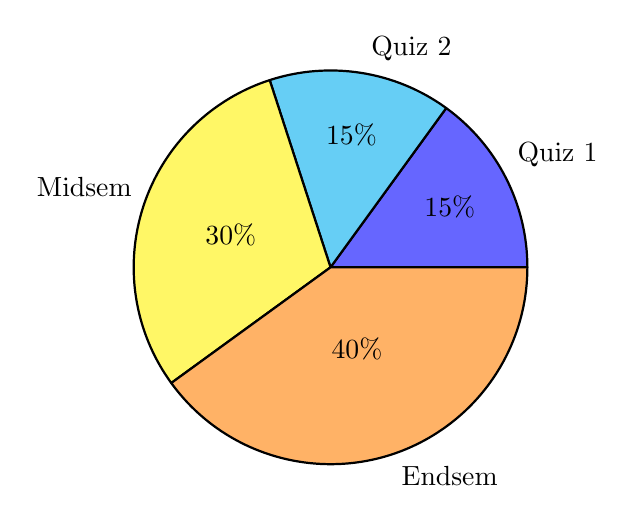
\begin{tikzpicture}
        \pie[radius=2.5]{15/Quiz 1, 15/Quiz 2, 30/Midsem, 40/Endsem}
        \end{tikzpicture}

        \subsubsection{CS231 (Lab)}
        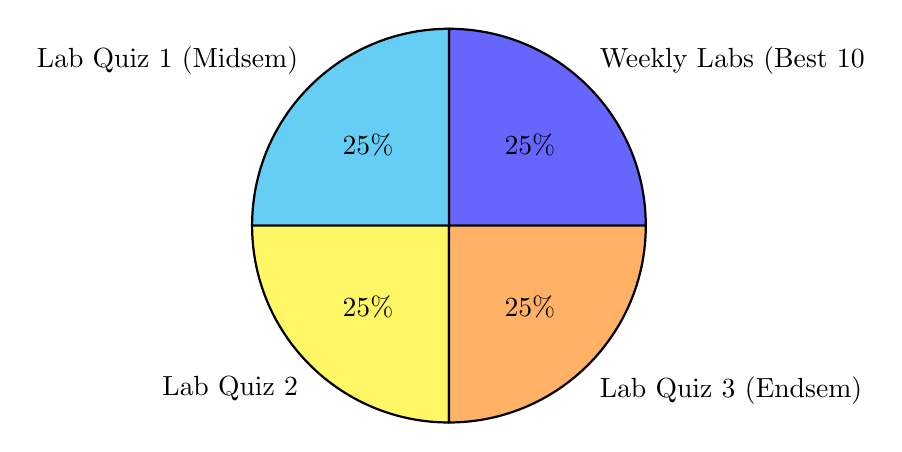
\begin{tikzpicture}
        \pie[radius=2.5]{25/Weekly Labs (Best 10/11 Inlabs), 25/Lab Quiz 1 (Midsem), 25/Lab Quiz 2, 25/Lab Quiz 3 (Endsem)}
        \end{tikzpicture}

\pagebreak


\section{Logic (CS228)}

    \subsection{Course websites}
    Course Content + Lecture slides: \\\url{https://www.cse.iitb.ac.in/~akshayss/courses/cs228-2026/cs228-2026.html}
    \\\\
    Class discussion (Piazza) : \\\url{https://piazza.com/class/ms4gwv81ixb3l0}

    \subsection{Help Sessions}
   Wednesdays, 3:30 - 4:30 PM (CC101, 103, 105)

    \subsection{Quizzes}
        Quiz 1 : Friday, 28th August 2026 (5:10-6:10 PM)\\
        Midsem : Wednesday, 16th September 2026 (11AM -1PM)
    \subsection{Grade Distribution}
    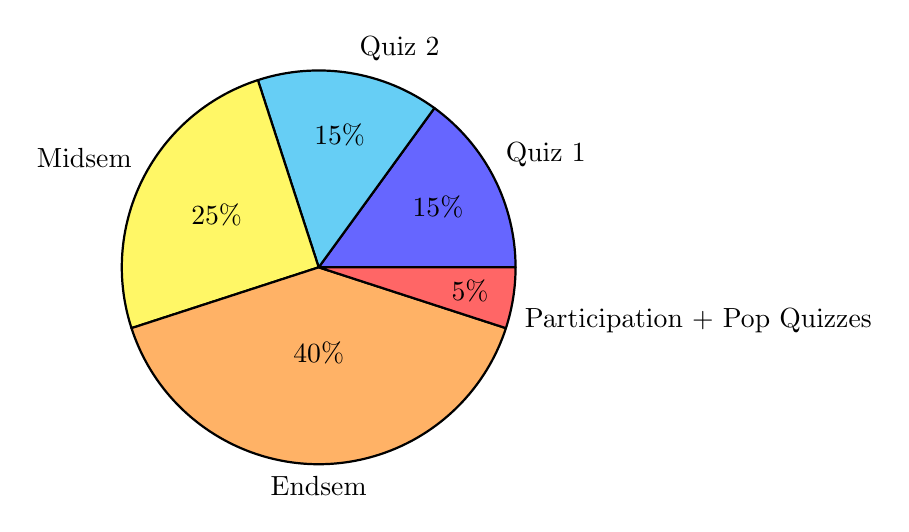
\begin{tikzpicture}
        \pie[radius=2.5]{15/Quiz 1, 15/Quiz 2, 25/Midsem, 40/Endsem, 5/Participation + Pop Quizzes}
    \end{tikzpicture}

\pagebreak


\section{DAI (CS215)}

    \subsection{Course websites}
    Class discussion (Piazza) : \\\url{https://piazza.com/class/ms1ll7021ih5yc}
    \\\\Lecture Slides (Piazza) : \\\url{https://piazza.com/class/ms1ll7021ih5yc/post/7#}

    \subsection{Help Sessions}
    Fridays, 5:15-6:15 PM (ESE107 or KReSIT or CC)

    \subsection{Quizzes}
        Midsem : Tuesday, 15th September 2026 (5-7 PM)
    \subsection{Grade Distribution}
\textit{Note that these are approximate values (Midsem : \textbf{25-30\%}, Endsem : \textbf{64-67\%}, Attendance + Participation : \textbf{5-7\%}, Assignments and Team Project : \textbf{Ungraded but high weightage for Endsem}).}\\\\
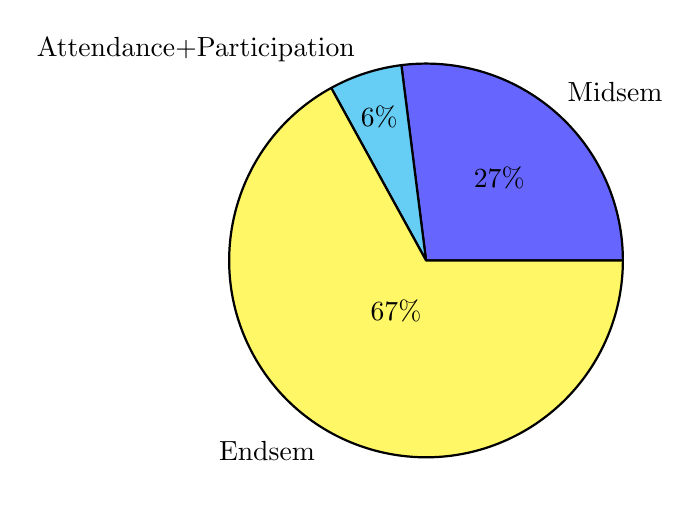
\begin{tikzpicture}
    \pie[radius=2.5]{
        27/Midsem,
        6/Attendance+Participation,
        67/Endsem
    }
\end{tikzpicture}



\end{document}
